\documentclass{beamer}

\usepackage{beamerthemeBerkeley}
%\usepackage{beamercolorthemeseahorse}
\usepackage{graphicx}
\usepackage[brazil]{babel}
\usepackage[latin1]{inputenc}

\logo{
\includegraphics[scale=0.2]{logo.png}}
%\logo{teste}

\title{An\'alise do \textit{sprint}}
\author{Ricardo Yamamoto Abe}
\date{}

\begin{document}

\beamertemplatetransparentcoveredmedium

\frame{\titlepage}

%\begin{frame}[shrink]
%\tableofcontents
%\end{frame}

\section{Introdu\c{c}\~ao}

\frame 
{
  \frametitle{Objetivos do \textit{sprint}}

  \begin{itemize}[<+->]
  \item Criar uma biblioteca de alto desempenho para Perl a partir do buscador
    original, utilizando \textit{Inline C}.
    
  \item Gerar a base de bairros lim\'itrofes a partir do cadastro
  geral e da base do DNE, utilizando a nova biblioteca.
  \end{itemize}
}

\section{Cria\c{c}\~ao da biblioteca}

\frame
{
  \frametitle{Estrutura original}

  \begin{figure}[h]
    \centering
    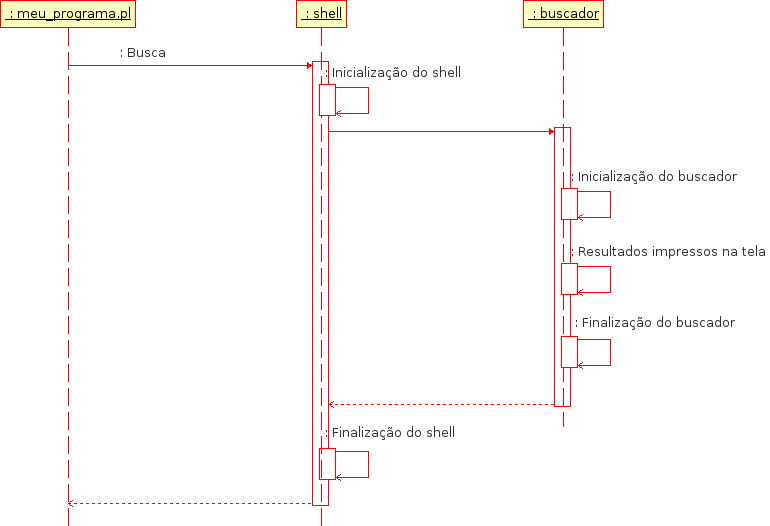
\includegraphics [scale=0.35,]{antigo.png}
  \end{figure}
}

\frame
{
  \frametitle{Estrutura nova}

  \begin{figure}[h]
    \centering
    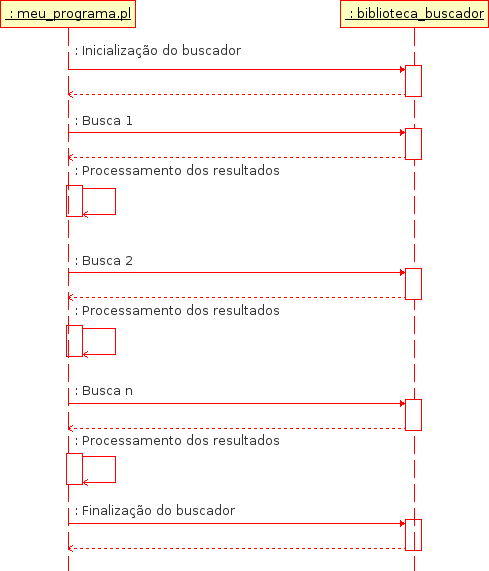
\includegraphics [scale=0.33]{novo.png}
  \end{figure}
}

\section{Processamento da base de bairros lim\'itrofes}

\frame
{
  \frametitle{Comparativo de desempenho na gera\c{c}\~ao da base de bairros lim\'itrofes -- estrutura original}

  \begin{center}
    \begin{tabular}{c|c}
      \hline
      N\'umero de processos & Desempenho\\
      \hline
      1 & 250 linhas/s\\
      2 & 416 linhas/s\\
      3 & 454 linhas/s\\
      4 & 481 linhas/s\\
      5 & 531 linhas/s\\
      \hline      
    \end{tabular}
  \end{center}
}

\frame
{
  \frametitle{Comparativo de desempenho na gera\c{c}\~ao da base de bairros lim\'itrofes -- estrutura nova}

  \begin{center}
    \begin{tabular}{c|c}
      \hline
      N\'umero de processos & Desempenho\\
      \hline
      1 & 2900 linhas/s\\
      2 & 4900 linhas/s\\
      \hline      
    \end{tabular}
  \end{center}
}

\frame
{
  \frametitle{Comparativo de desempenho na gera\c{c}\~ao da base de bairros lim\'itrofes}

  \begin{figure}[h]
    \centering
    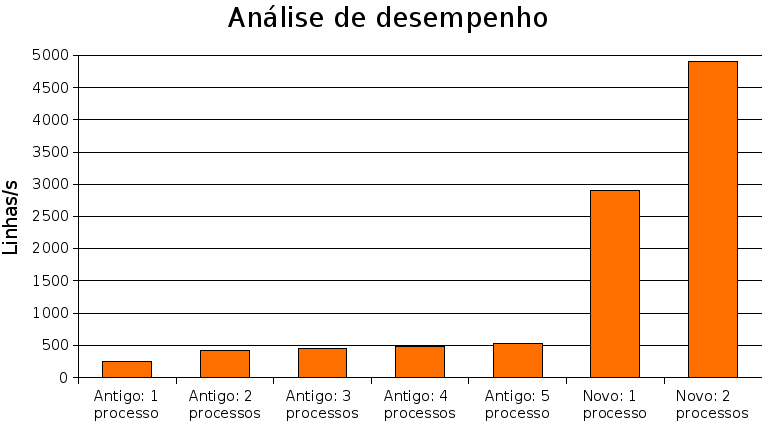
\includegraphics [scale=0.35,]{grafico.png}
  \end{figure}
}

\frame
{
  \frametitle{Comparativo de desempenho na gera\c{c}\~ao de base de bairro lim\'itrofes}

  \begin{itemize}[<+->]
    \item Total de endere\c{c}os obtidos do cadastro geral: 334.851.226 registros.
    \item Tempo estimado para processamento na estrutura original: 175,2 horas (7,3 dias).
    \item Tempo para processamento na estrutura nova: 15 horas (0,6 dia).
  \end{itemize}
}

\end{document}
